\documentclass{report}

\usepackage{amsmath}
\usepackage{geometry}
\usepackage{amsfonts}
\usepackage[english]{babel}
\usepackage{amssymb}
\usepackage{graphicx}
\usepackage{float}
\usepackage{hyperref}
\usepackage{multirow}
\usepackage{pdflscape}
\usepackage{caption}
\usepackage{pdflscape}
\usepackage{outlines}
\usepackage{subcaption}
\usepackage{enumerate}

\usepackage{tabularx, booktabs}

\usepackage{standalone}

\usepackage[autostyle, english = american]{csquotes}
\MakeOuterQuote{"}

\usepackage{comment}

\newcommand{\tabnotes}[2]{\bottomrule \multicolumn{#1}{@{}p{0.95\linewidth}@{}}{\footnotesize #2 }\end{tabular}\end{table}}

\title{Defense Spending Spillovers}
\author{Isaac Liu}
\date{\today}

\setlength{\parindent}{0pt}
\setlength{\parskip}{0.5em}

\hypersetup{
    colorlinks=true,
    linkcolor=blue,
    filecolor=magenta,      
    urlcolor=cyan,
}

\begin{document}

	\maketitle

	\newpage \clearpage

    \section*{Military Expenditure Data}

    Our data on military expenditure as a percentage of GDP comes from SIPRI, the Stockholm International
	Peace Research Institute.

	\begin{figure}[h!]
		\centering
		\caption{Military Expenditure as Percentage of GDP Time Series for Countries}
		\label{Milex_GDP_Time_Series}	
		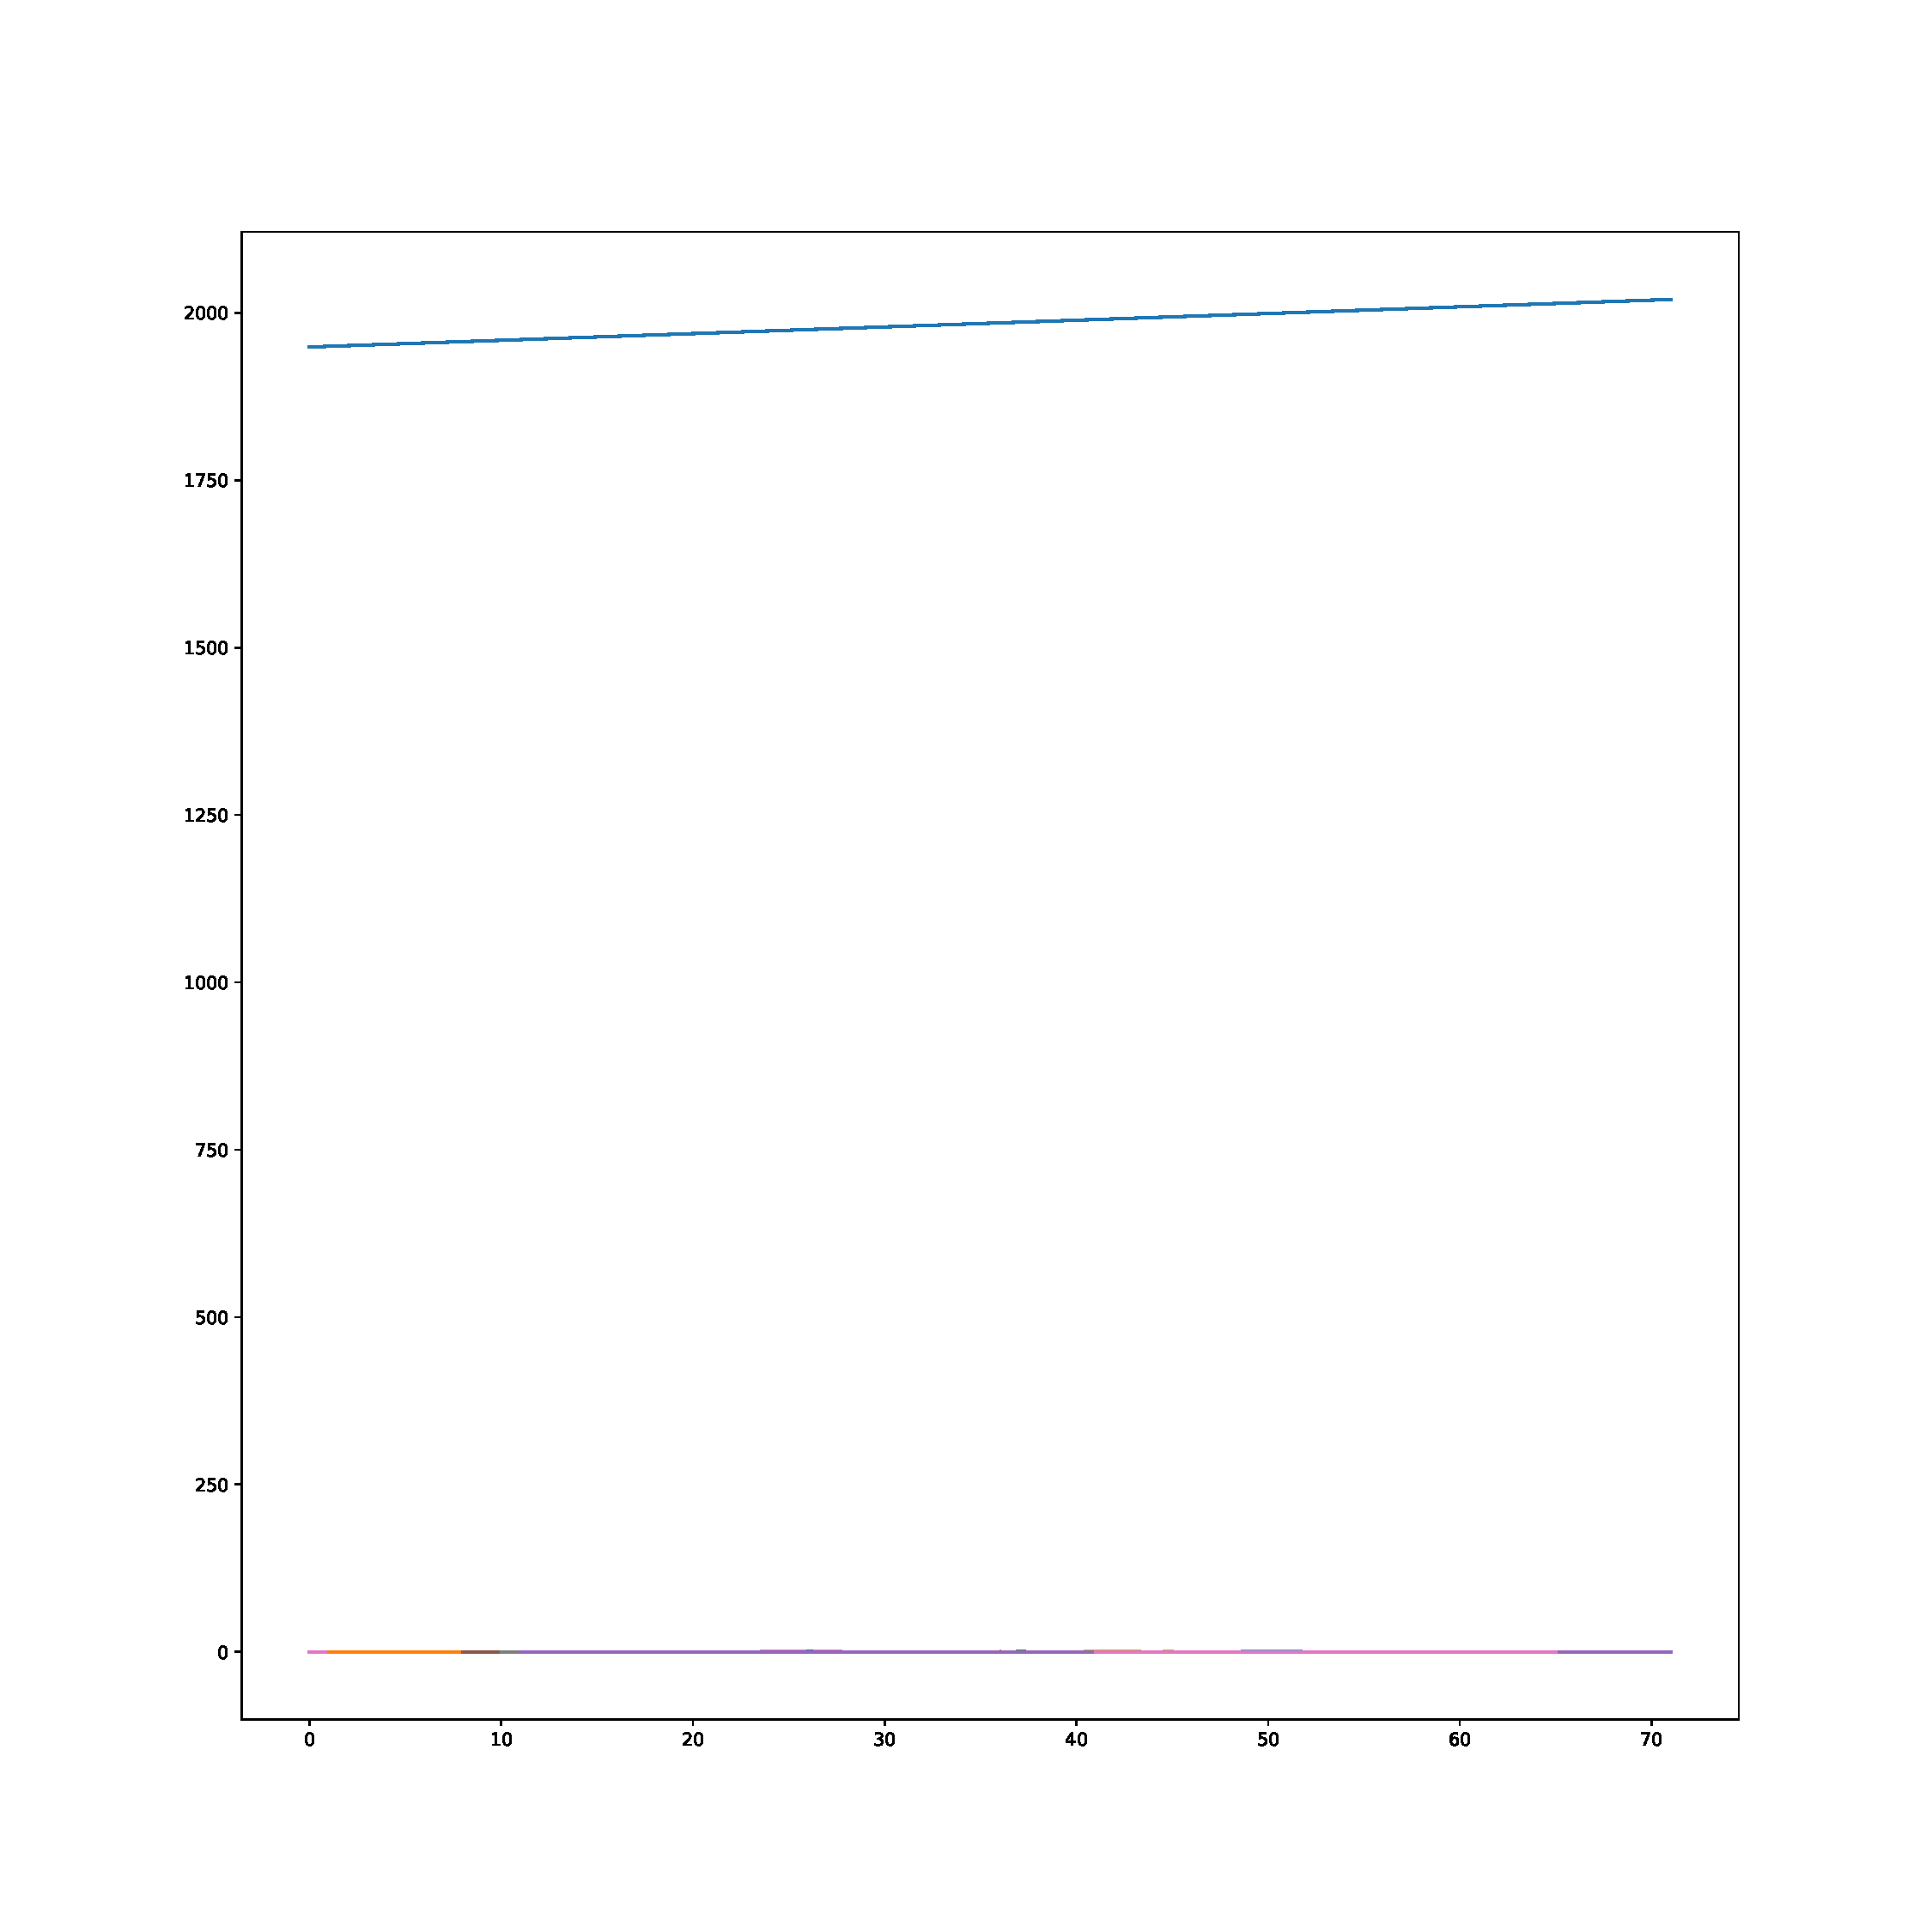
\includegraphics[width=\linewidth,keepaspectratio=true]{../Output/Figures/Milex_GDP_Time_Series.pdf}
	\end{figure}

	\begin{figure}[h!]
		\centering
		\caption{Correlations Between Country Military Spending}
		\label{Milex_Correlations}	
		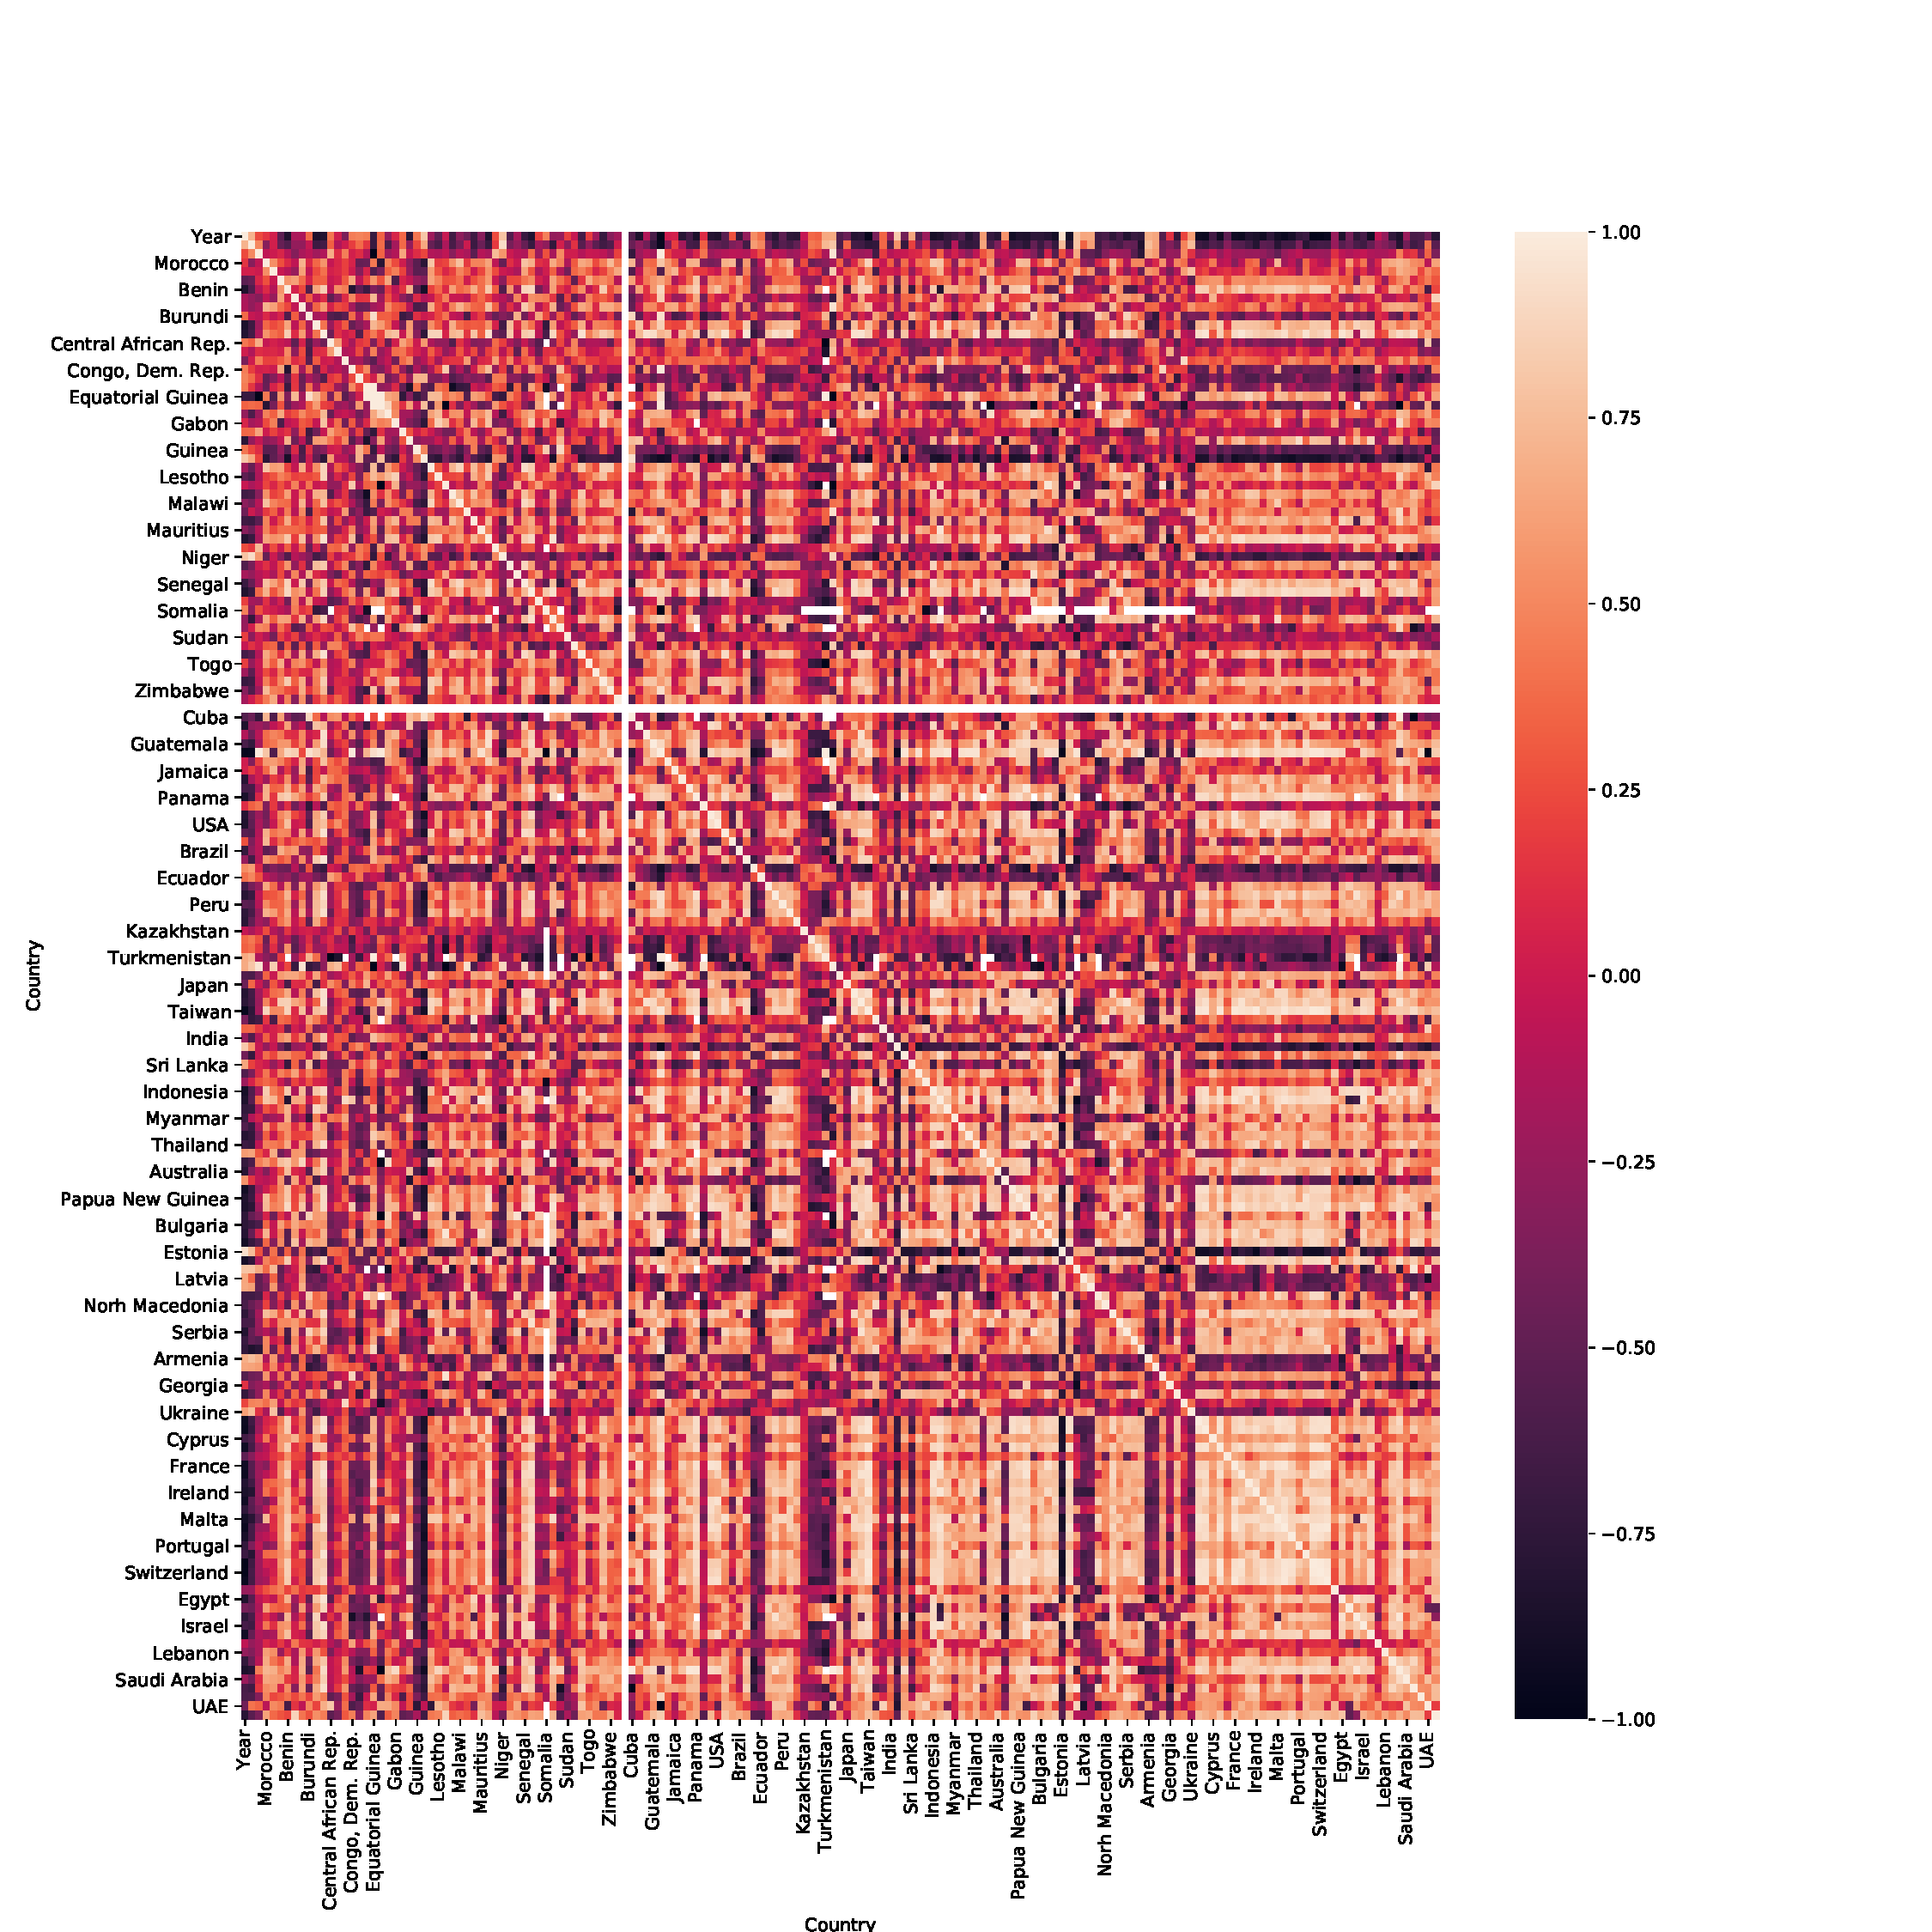
\includegraphics[width=\linewidth,keepaspectratio=true]{../Output/Figures/Milex_Correlations.pdf}
	\end{figure}

    \section*{The Missing Values Problem}

    In order to use PCA and the LASSO, we need to figure out a way to handle missing values in the panel. Here I interpolate values between data points where we have spending information for a country, and also restrict the sample to observations after 1995.

	\begin{figure}[h!]
		\centering
		\caption{Missing Values Before Interpolation}
		\label{SIPRI_Missing_Values}	
		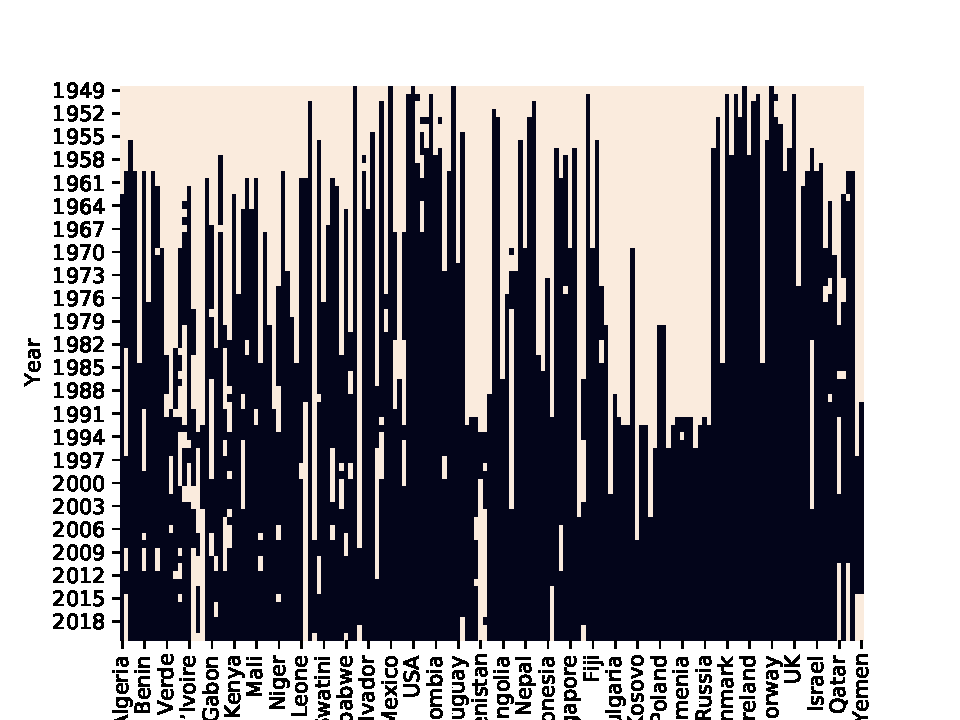
\includegraphics[width=\linewidth,keepaspectratio=true]{../Output/Figures/SIPRI_Missing_Values.pdf}
	\end{figure}

	\begin{figure}[h!]
		\centering
		\caption{Missing Values After Interpolation and Sample Restriction}
		\label{SIPRI_Missing_Values_Inter_Post_1995}	
		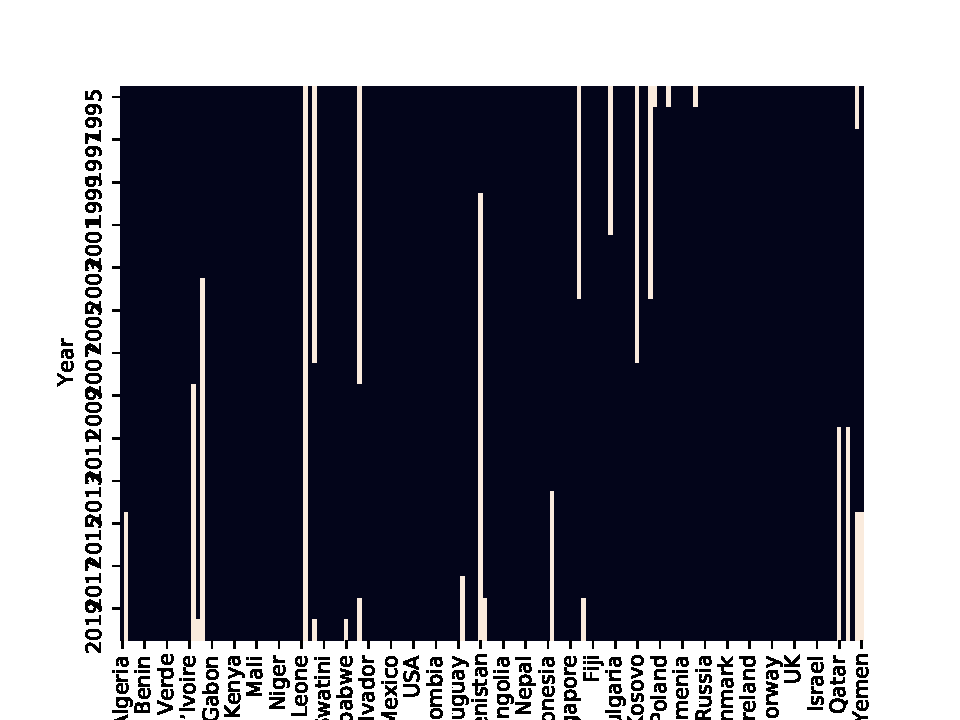
\includegraphics[width=\linewidth,keepaspectratio=true]{../Output/Figures/SIPRI_Missing_Values_Interpolate_Post_1995.pdf}
	\end{figure}

    \newpage \clearpage

    \section*{PCA Results}

    I performed a PCA to see if there were components which explained a large amount of the variation in spending across countries and over time.

	\begin{figure}[h!]
		\centering
		\caption{Military Spending PCA Loadings}
		\label{Milex_Loadings}	
		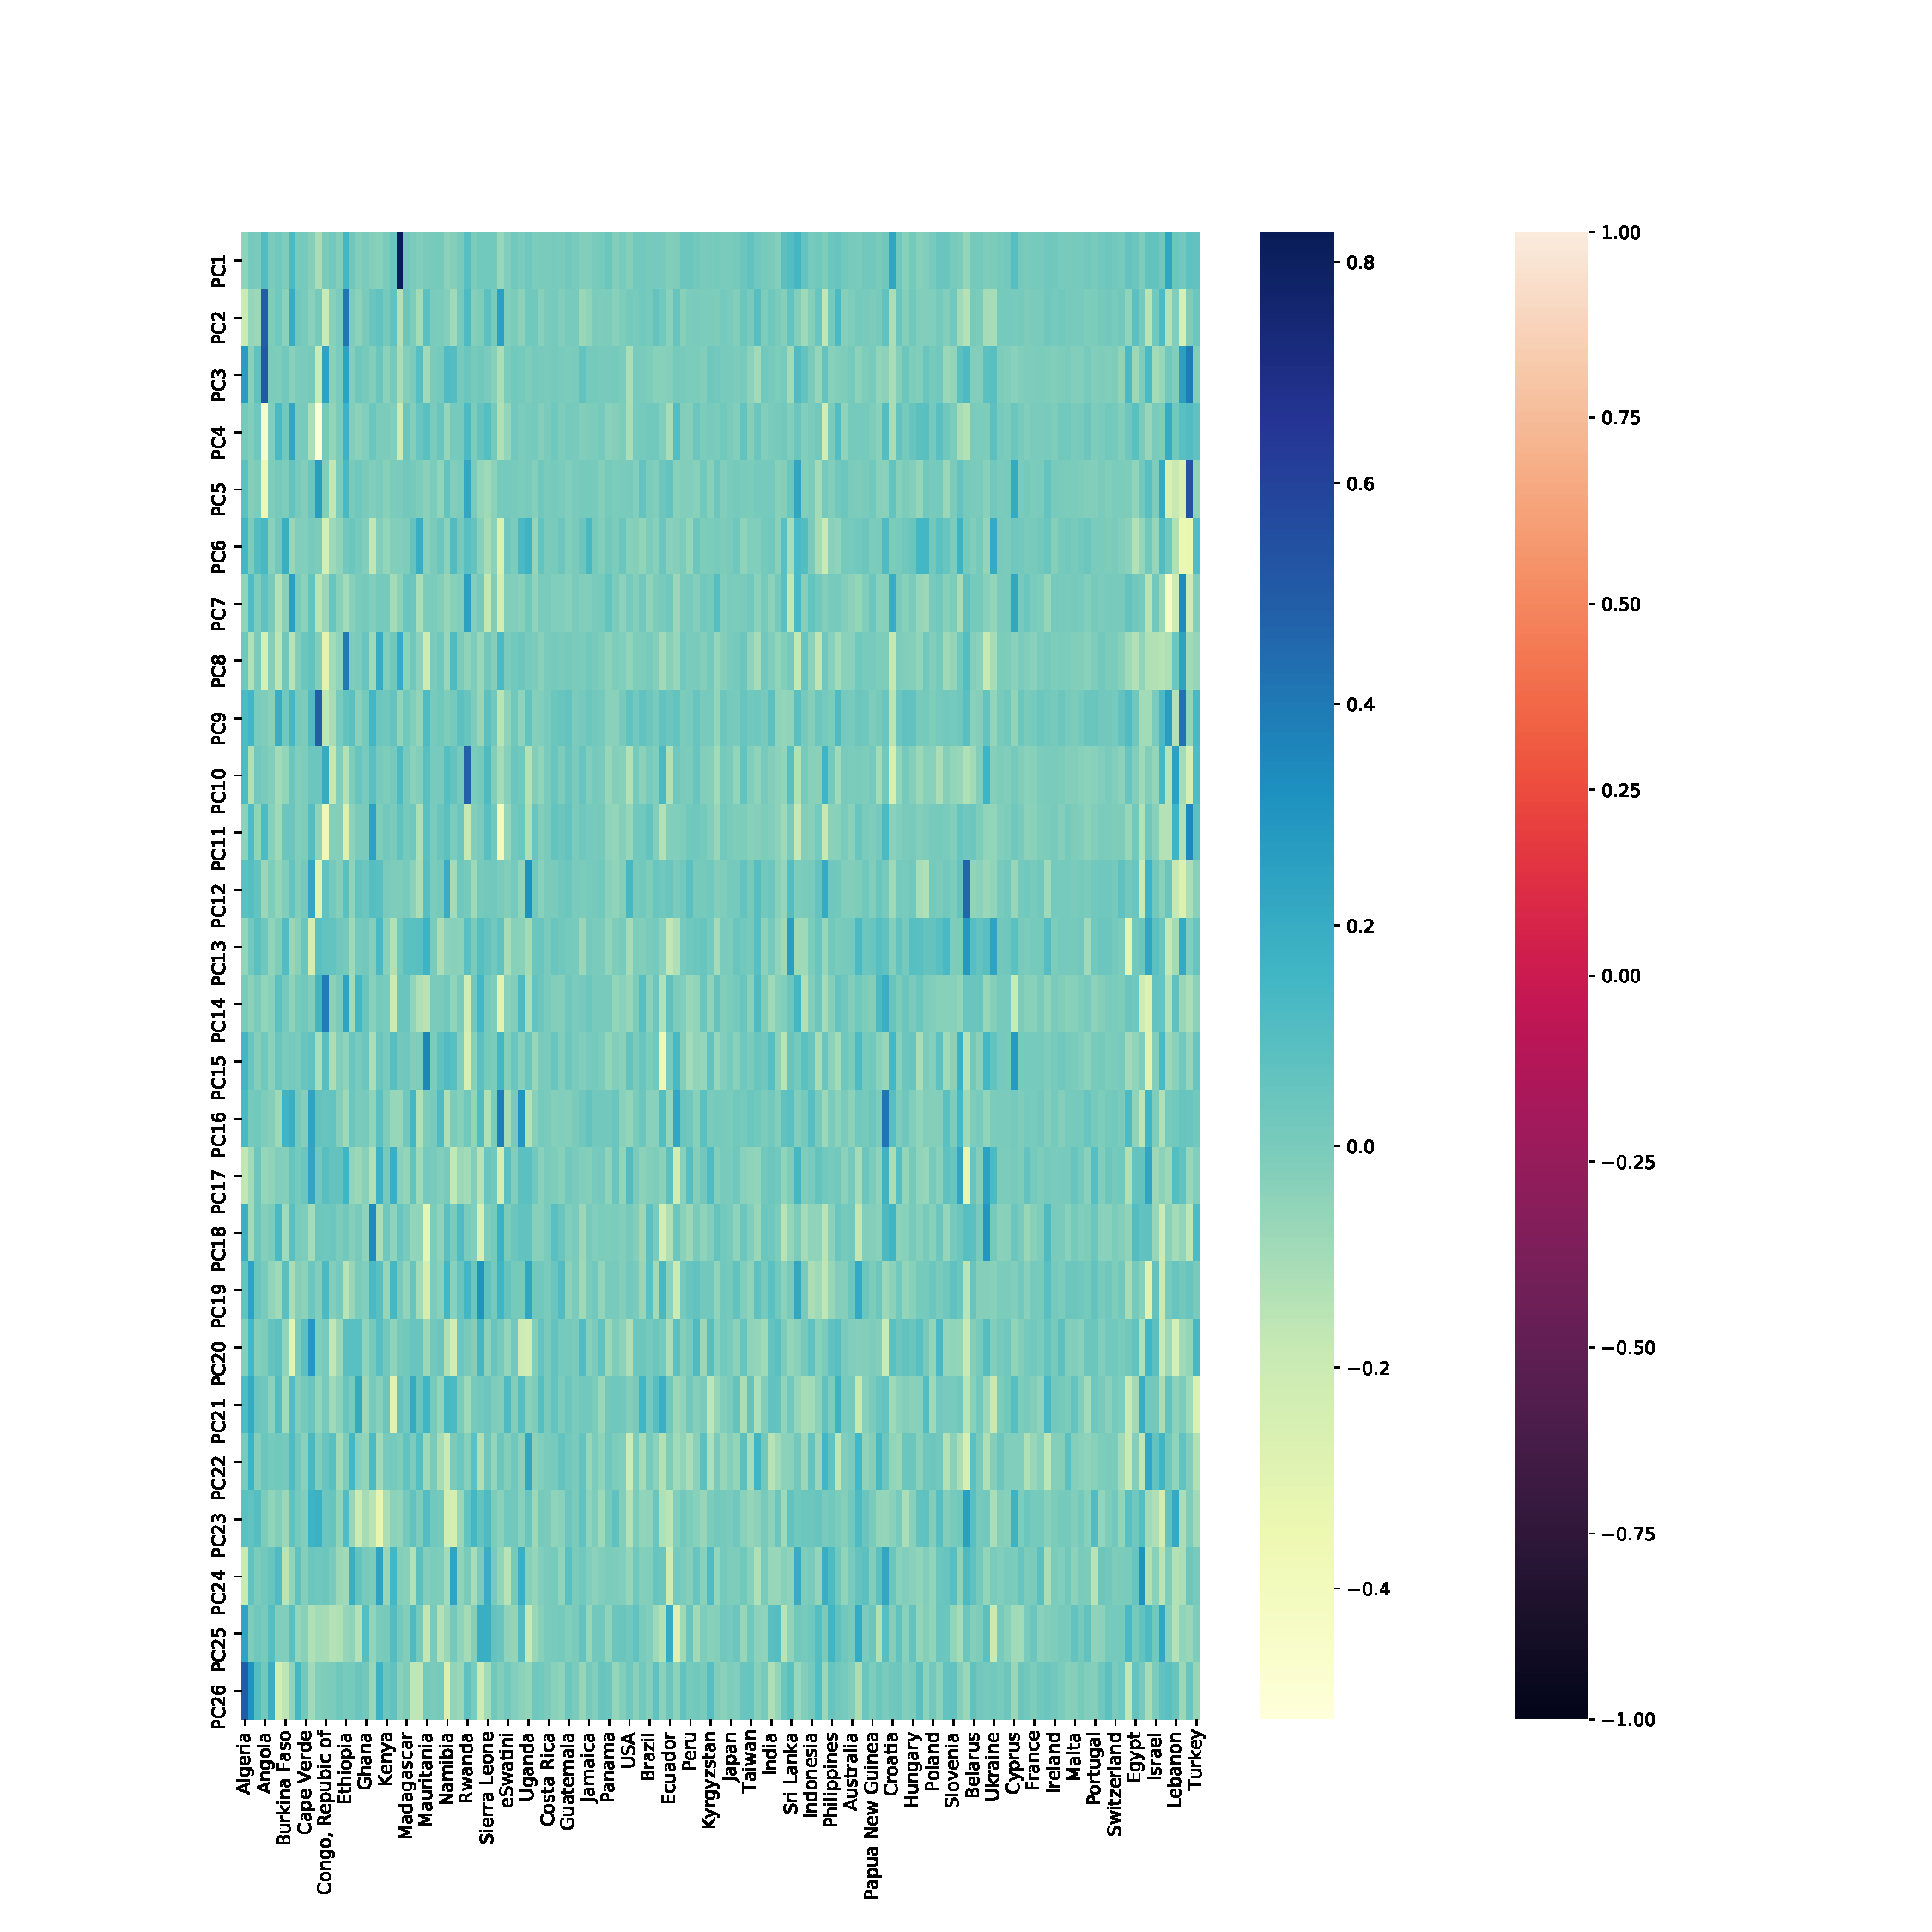
\includegraphics[width=\linewidth,keepaspectratio=true]{../Output/Figures/Milex_Loadings.pdf}
	\end{figure}

    The data is very well summarized with very few principal components.

	\begin{figure}[h!]
		\centering
		\caption{Military Spending PCA Share of Variance Explained}
		\label{Milex_PC_Share_Explained}	
		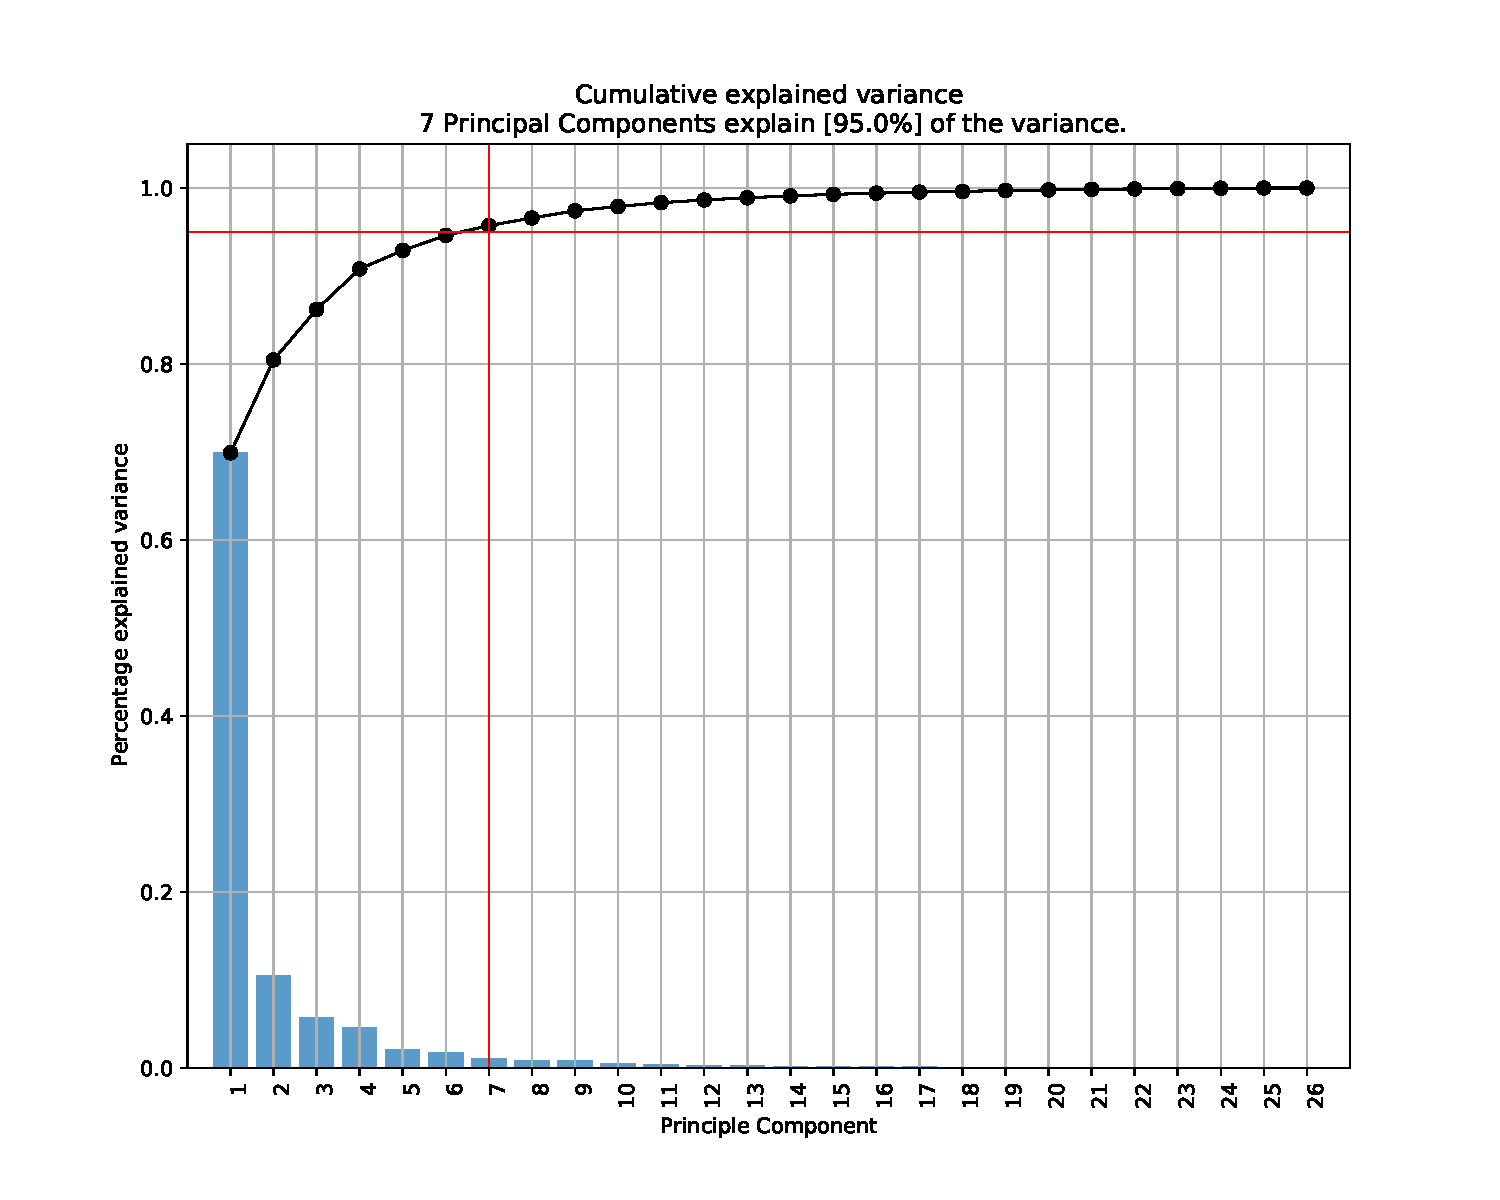
\includegraphics[width=\linewidth,keepaspectratio=true]{../Output/Figures/Milex_PC_Share_Explained.pdf}
	\end{figure}

\end{document}